\documentclass[superscriptaddress,onecolumn,floatfix]{revtex4-2}

\usepackage{graphicx}
\usepackage{epsfig}
\usepackage{color}
\usepackage{amssymb}
\usepackage{amsmath}
\usepackage{array}
\usepackage[loose]{units}
\usepackage[french]{babel}
\usepackage[unicode]{hyperref}
\usepackage{cleveref}
\usepackage{braket}
\usepackage[caption=false]{subfig}
\usepackage{letltxmacro}

\pdfcompresslevel=9

\LetLtxMacro{\ORIGselectlanguage}{\selectlanguage}
\makeatletter
\DeclareRobustCommand{\selectlanguage}[1]{%
    \@ifundefined{alias@\string#1}
      {\ORIGselectlanguage{#1}}
      {\begingroup\edef\x{\endgroup
         \noexpand\ORIGselectlanguage{\@nameuse{alias@#1}}}\x}%
}
\newcommand{\definelanguagealias}[2]{%
  \@namedef{alias@#1}{#2}%
}
\makeatother

\definelanguagealias{fr}{french}


\begin{document}
\selectlanguage{fr}

\begin{abstract}
Ce guide vous guide à travers les étapes nécessaires pour installer le kit de préconditionnement de l'unité principale dans votre Ioniq 6 2023-2025. 
\begin{description}
  \item[Étape 1 : Débranchez le 12 V] 
  \item[Étape 2 : Couper]
  \item[Étape 3 : Connexion du faisceau] 
  \item[Étape 4 : Montage OBD] 
  \item[Étape 4.5 : Plug-in WiCAN] 
\end{description}
\end{abstract}
\title{Guide d'installation du kit de préconditionnement : Ioniq 6}
\author{Ioniq Guy}
\author{Boutique de boutons Electroniq}
\email{support@electroniqbuttons.com}
% \affiliation{\GOE}
% \author{Benjamin J. McMorran}
% \email{mcmorran@uoregon.edu}
% \affiliation{\UO}
\date{\today}

\maketitle

\begin{figure}[h]
  \subfloat[]{\label{subfig:overview:harness}
  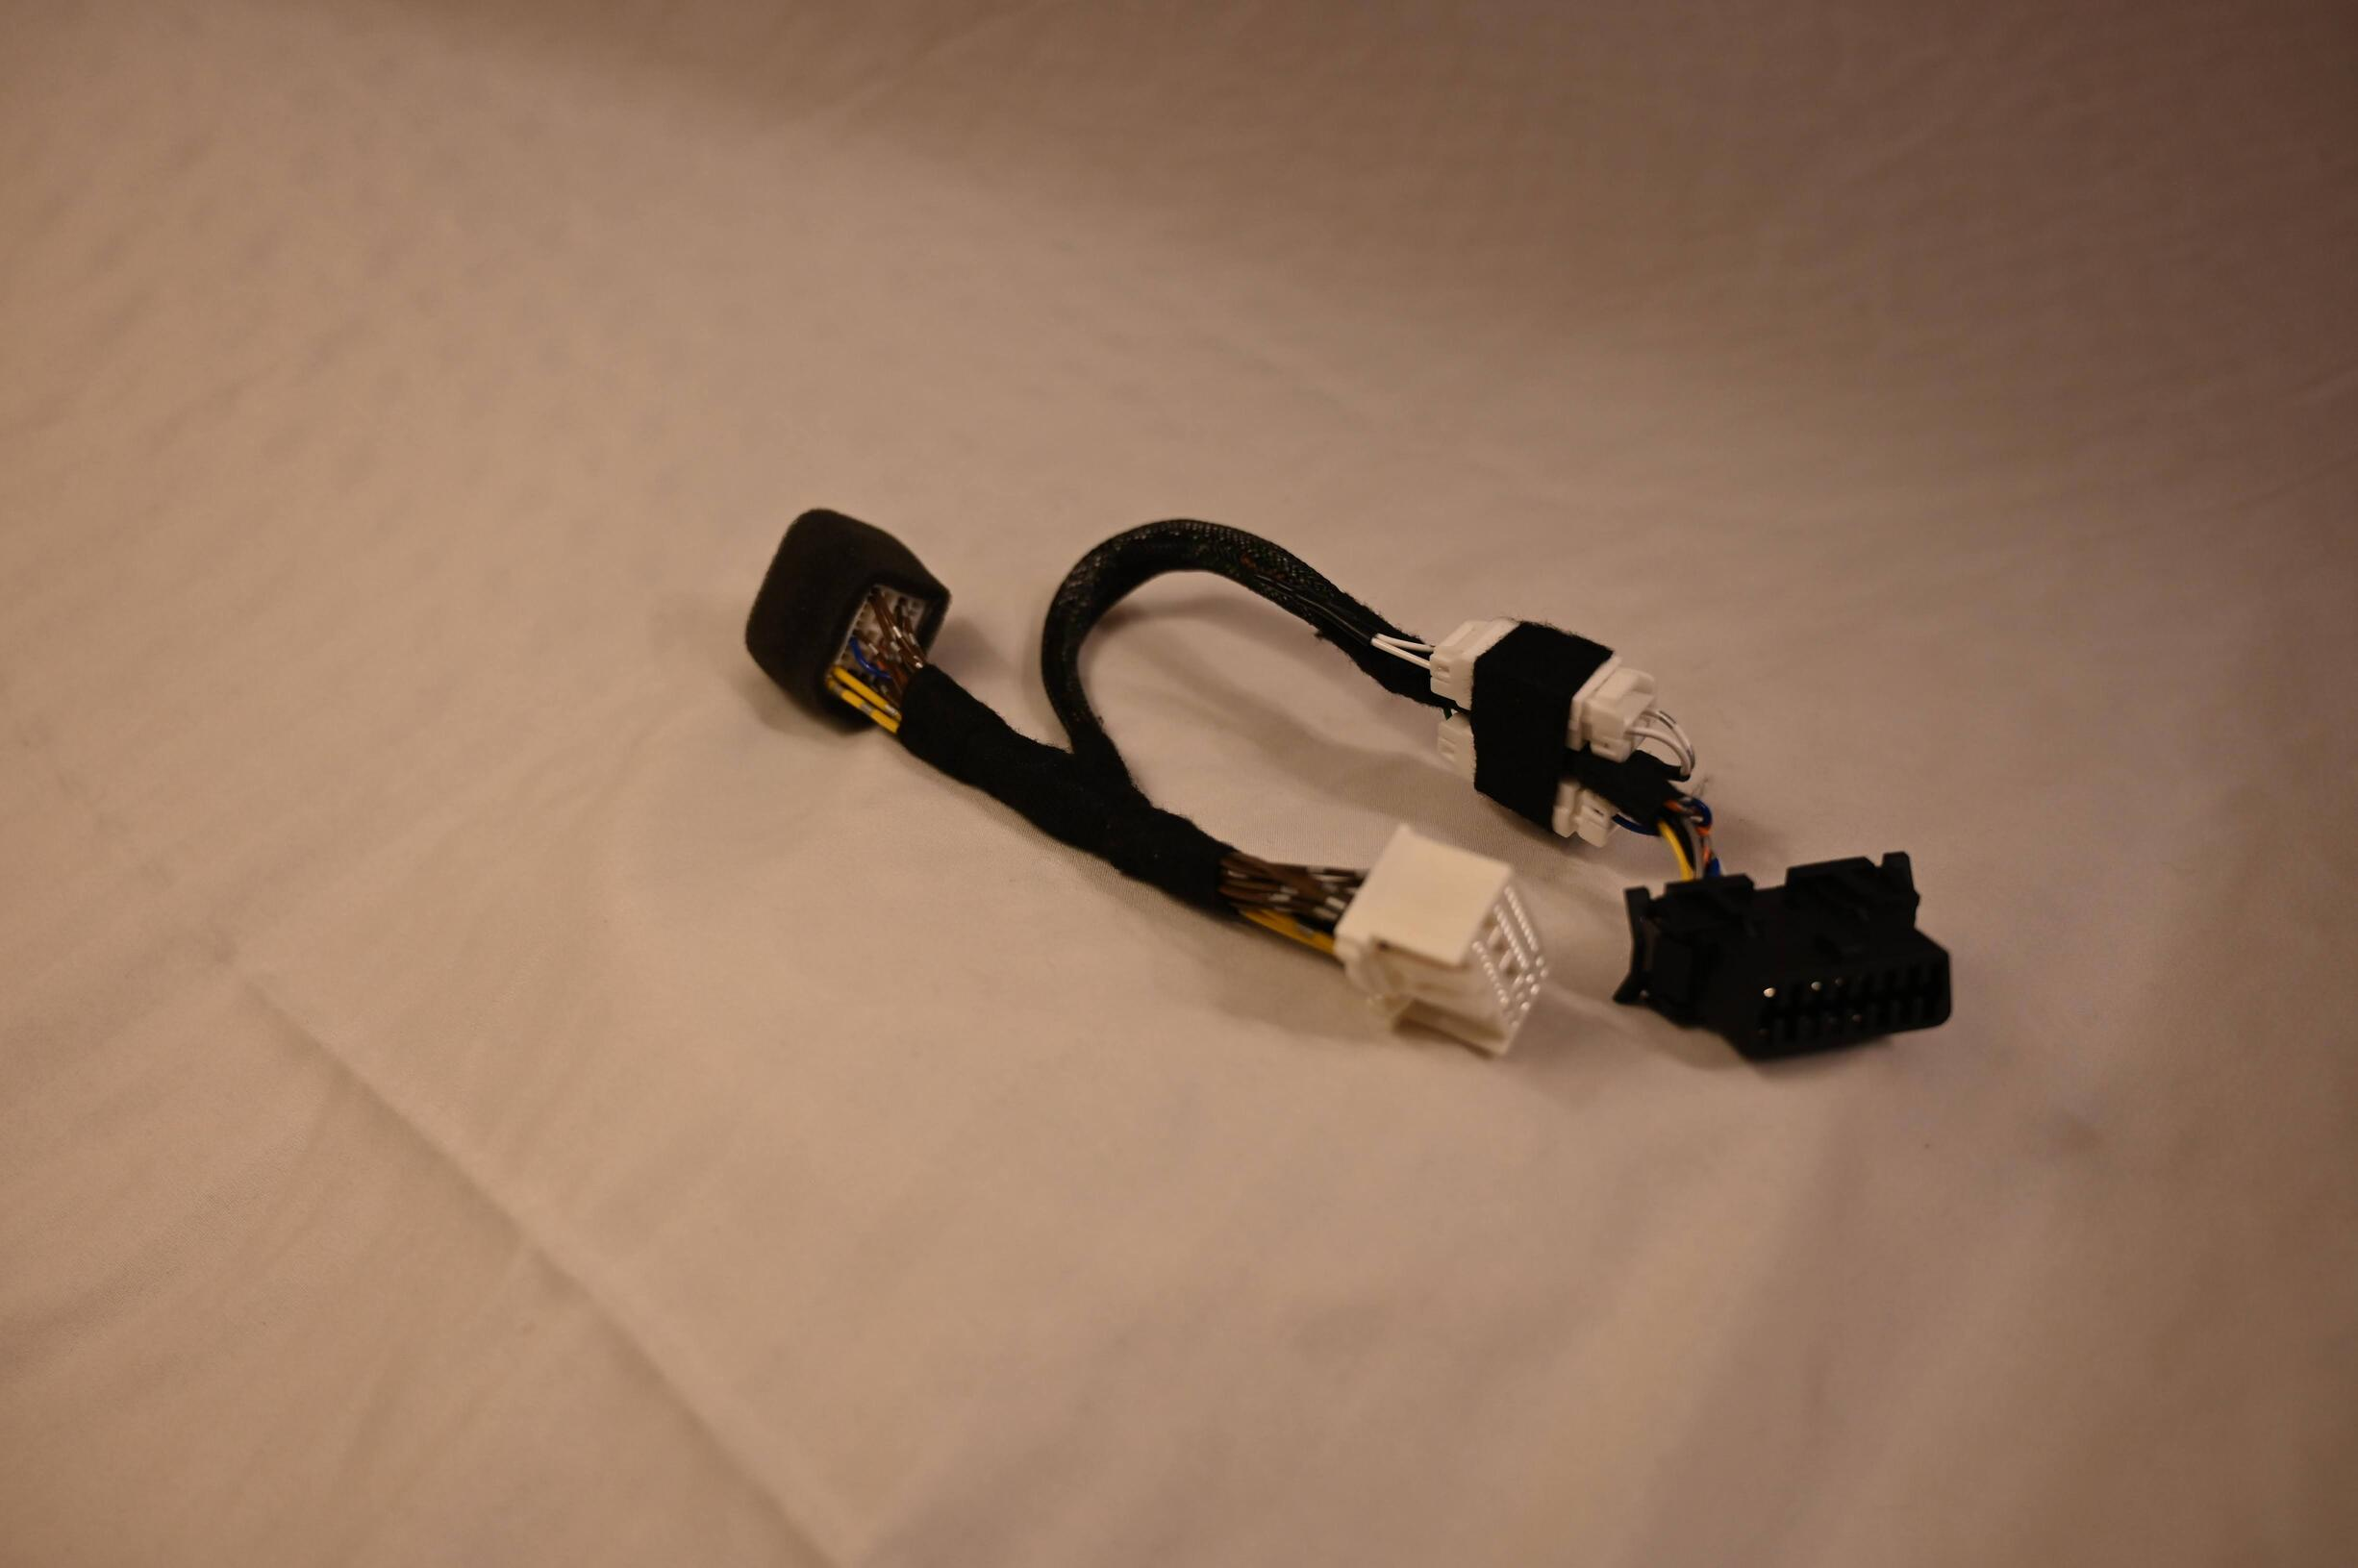
\includegraphics[height=1.95in]{../../../harnesses/head_unit_MITM/photos/whole_harness.jpg} } \\
  % \subfloat[]{\label{subfig:overview:trim}
  % 
\includegraphics[width=6in]{photos/overview_labeled.jpg} }
   \caption{(a) Harnais d'homme au milieu. \label{fig:overview}}
\end{figure}

\section{Introduction}
  Le but de ce guide est d'illustrer les instructions étape par étape pour l'installation du kit de préconditionnement de l'unité principale, ou simplement du faisceau d'homme au milieu (MITM) de l'unité principale, illustré dans la figure \ref{subfig:overview:harness}. Dans la rubrique \ref{sect:1}, nous décrivons le processus de retrait des garnitures pour accéder à l'unité principale. Dans la rubrique \ref{sect:2}, nous décrivons le processus de branchement du harnais. Dans la rubrique \ref{sect:3}, nous montrons la fixation du port OBD et comment brancher le microcontrôleur. 

Outils nécessaires :
\begin{enumerate}
  \item Douille de 10 mm ou clé à molette pour batterie 12 V (non incluse)
  \item Outils de suppression de garniture (inclus si sélectionnés)
\end{enumerate}

Composants du kit :
\begin{enumerate}
  \item Harnais de l'unité principale
  \item WiCAN
  \item Support de montage OBD de 70 mm
  \item Ruban adhésif double face de 70 mm (deux pièces incluses pour la redondance)
  \item 4 attaches zippées
\end{enumerate}

\section{Étape 1 : Retirez la borne négative 12 V} \label{sect:0}
Tout d’abord, débranchez toujours la batterie 12V avant de retirer les connecteurs électriques ! Le retrait d'un connecteur électrique sous tension pourrait provoquer une décharge et détruire un connecteur ou un calculateur dans votre voiture.

Instructions étape par étape :
\begin{enumerate}
  \item Capot ouvert % (Figure \ref{subfig:12V:hood})
  \item Frunk ouvert (Figure \ref{subfig:12V:frunk})
  \item Retirer le revêtement du panneau 12V % (Figure \ref{subfig:12V:panel})
  \item Desserrez l'écrou du côté négatif avec une douille de 10 mm % (Figure \ref{subfig:12V:nut})
  \item Retirer la borne négative % (Figure \ref{subfig:12V:terminal})
\end{enumerate}

\begin{figure}[h]
  % \subfloat[]{\label{subfig:12V:hood}
  % 
\includegraphics[height=1.5in]{photos/open_hood.jpg} } 
  % \subfloat[]{\label{subfig:12V:panel}
  % 
\includegraphics[height=1.5in]{photos/remove_panel.jpg} }  \\
  % \subfloat[]{\label{subfig:12V:nut}
  % 
\includegraphics[height=1.5in]{photos/loosen_nut.jpg} } 
  % \subfloat[]{\label{subfig:12V:terminal}
  % 
\includegraphics[height=1.5in]{photos/disconnect_terminal.jpg} } 
  \subfloat[]{\label{subfig:12V:frunk}
  \includegraphics[height=1.5in]{photos/frunk.jpg} } 
  \caption{(a) Le coffre ouvert. \label{fig:12V}}
   % \caption{(a) Open the hood. (b) Remove panel covering 12V. (c) Loosen nut on negative terminal. (d) Remove negative terminal. \label{fig:12V}}
\end{figure}

\section{Étape 2 : Couper} \label{sect:1}
Le but ici est d'accéder au coffre au trésor : l'unité principale. Il se trouve derrière un seul panneau de garniture appelé Crash Pad Under Cover, marqué d'un X sur la figure. \ref{fig:step1}.
\begin{figure}[h]
  \subfloat[]{\label{subfig:step1:X}
  \includegraphics[height=2.95in]{photos/x_marks_HU.jpg} } 
   \caption{X marque l'unité principale. \label{fig:step1}}
\end{figure}

Instructions étape par étape :
\begin{enumerate}
  \item Retirez le coussin de protection sous le couvercle (Figure \ref{subfig:trim:crash_pad_under_cover}): 
    \begin{enumerate}
      \item Utilisez un outil de retrait de garniture pour faire levier doucement afin d'exposer l'un des trois clips (Figure \ref{subfig:trim:open})
      \item Appuyez sur la languette du clip, indiquée par le pouce de Corbin sur la figure \ref{subfig:trim:open}, pour libérer le clip
    \end{enumerate}
  \item Retirez les vis qui maintiennent l'unité principale en place (Figure \ref{subfig:trim:HU_screws})
\end{enumerate}

\begin{figure}[h]
  \subfloat[]{\label{subfig:trim:crash_pad_under_cover}
  \includegraphics[height=1.5in]{photos/harness_installed_1.jpg} } 
  \subfloat[]{\label{subfig:trim:open}
  \includegraphics[height=1.5in]{photos/panel_open.jpg} } 
  \subfloat[]{\label{subfig:trim:HU}
  \includegraphics[height=1.5in]{photos/HU_exposed.jpg} } 
  \subfloat[]{\label{subfig:trim:HU_screws}
  \includegraphics[height=1.5in]{photos/reinstalling_HU.jpg} } 
   \caption{(a) Crash pad sous le couvercle. (b) Dépose du crash pad sous le couvercle. (c) Unité principale exposée. (d) Retrait des vis maintenant l'unité principale en place. \label{fig:trim}}
\end{figure}


\section{Étape 3 : Connexion du faisceau} \label{sect:2}
Cette étape couvre l'installation du harnais dans l'unité principale. 

Instructions étape par étape :
\begin{enumerate}
  \item Identifiez le connecteur gris d'origine de l'unité principale femelle (Figure \ref{subfig:harness:headunit_oe_connectors})
  \item Retirez-le en appuyant sur le clip et en tirant vers le bas 
  \item Insérez le connecteur femelle que vous avez retiré dans le côté mâle du faisceau (Figure \ref{subfig:harness:harness_male_in})
  \item Insérez le côté femelle du harnais dans l'unité principale (Figure \ref{subfig:harness:harness_in})
\end{enumerate}

\begin{figure}[h]
  \subfloat[]{\label{subfig:harness:female}
  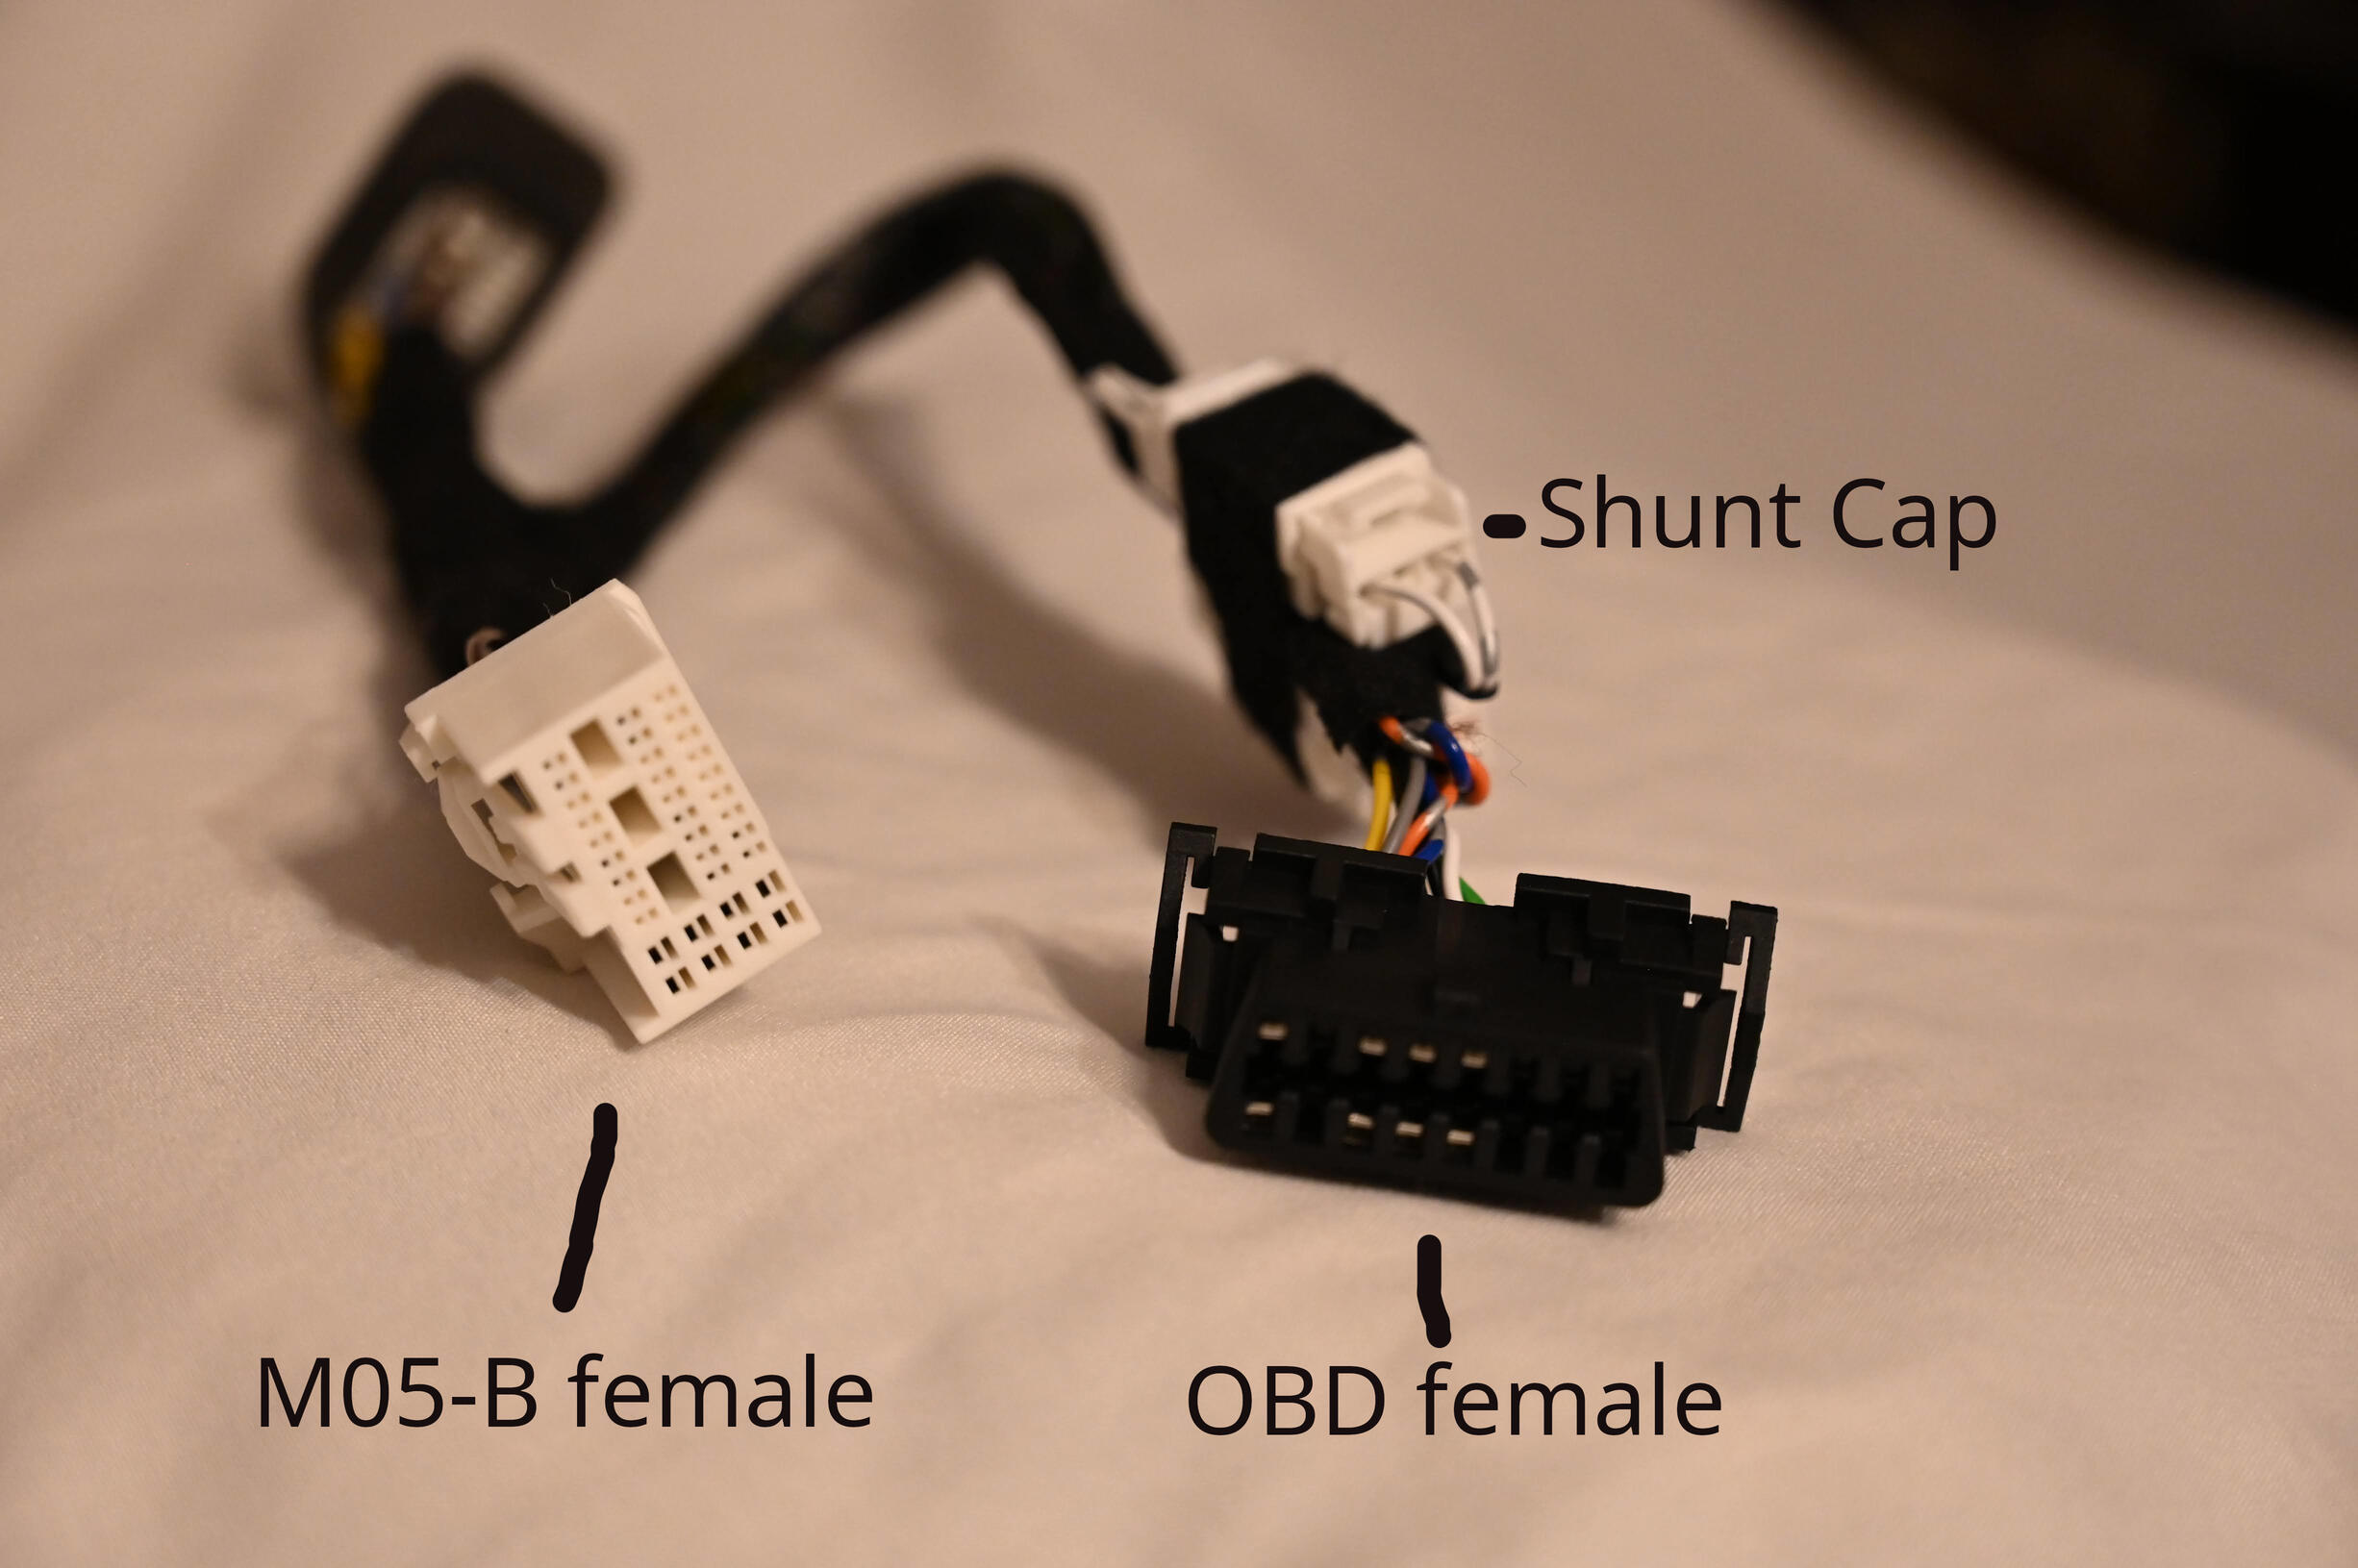
\includegraphics[height=1.5in,angle=0]{../../../harnesses/head_unit_MITM/photos/labeled_connectors_MITM_harness.jpg} } 
  \subfloat[]{\label{subfig:harness:male}
  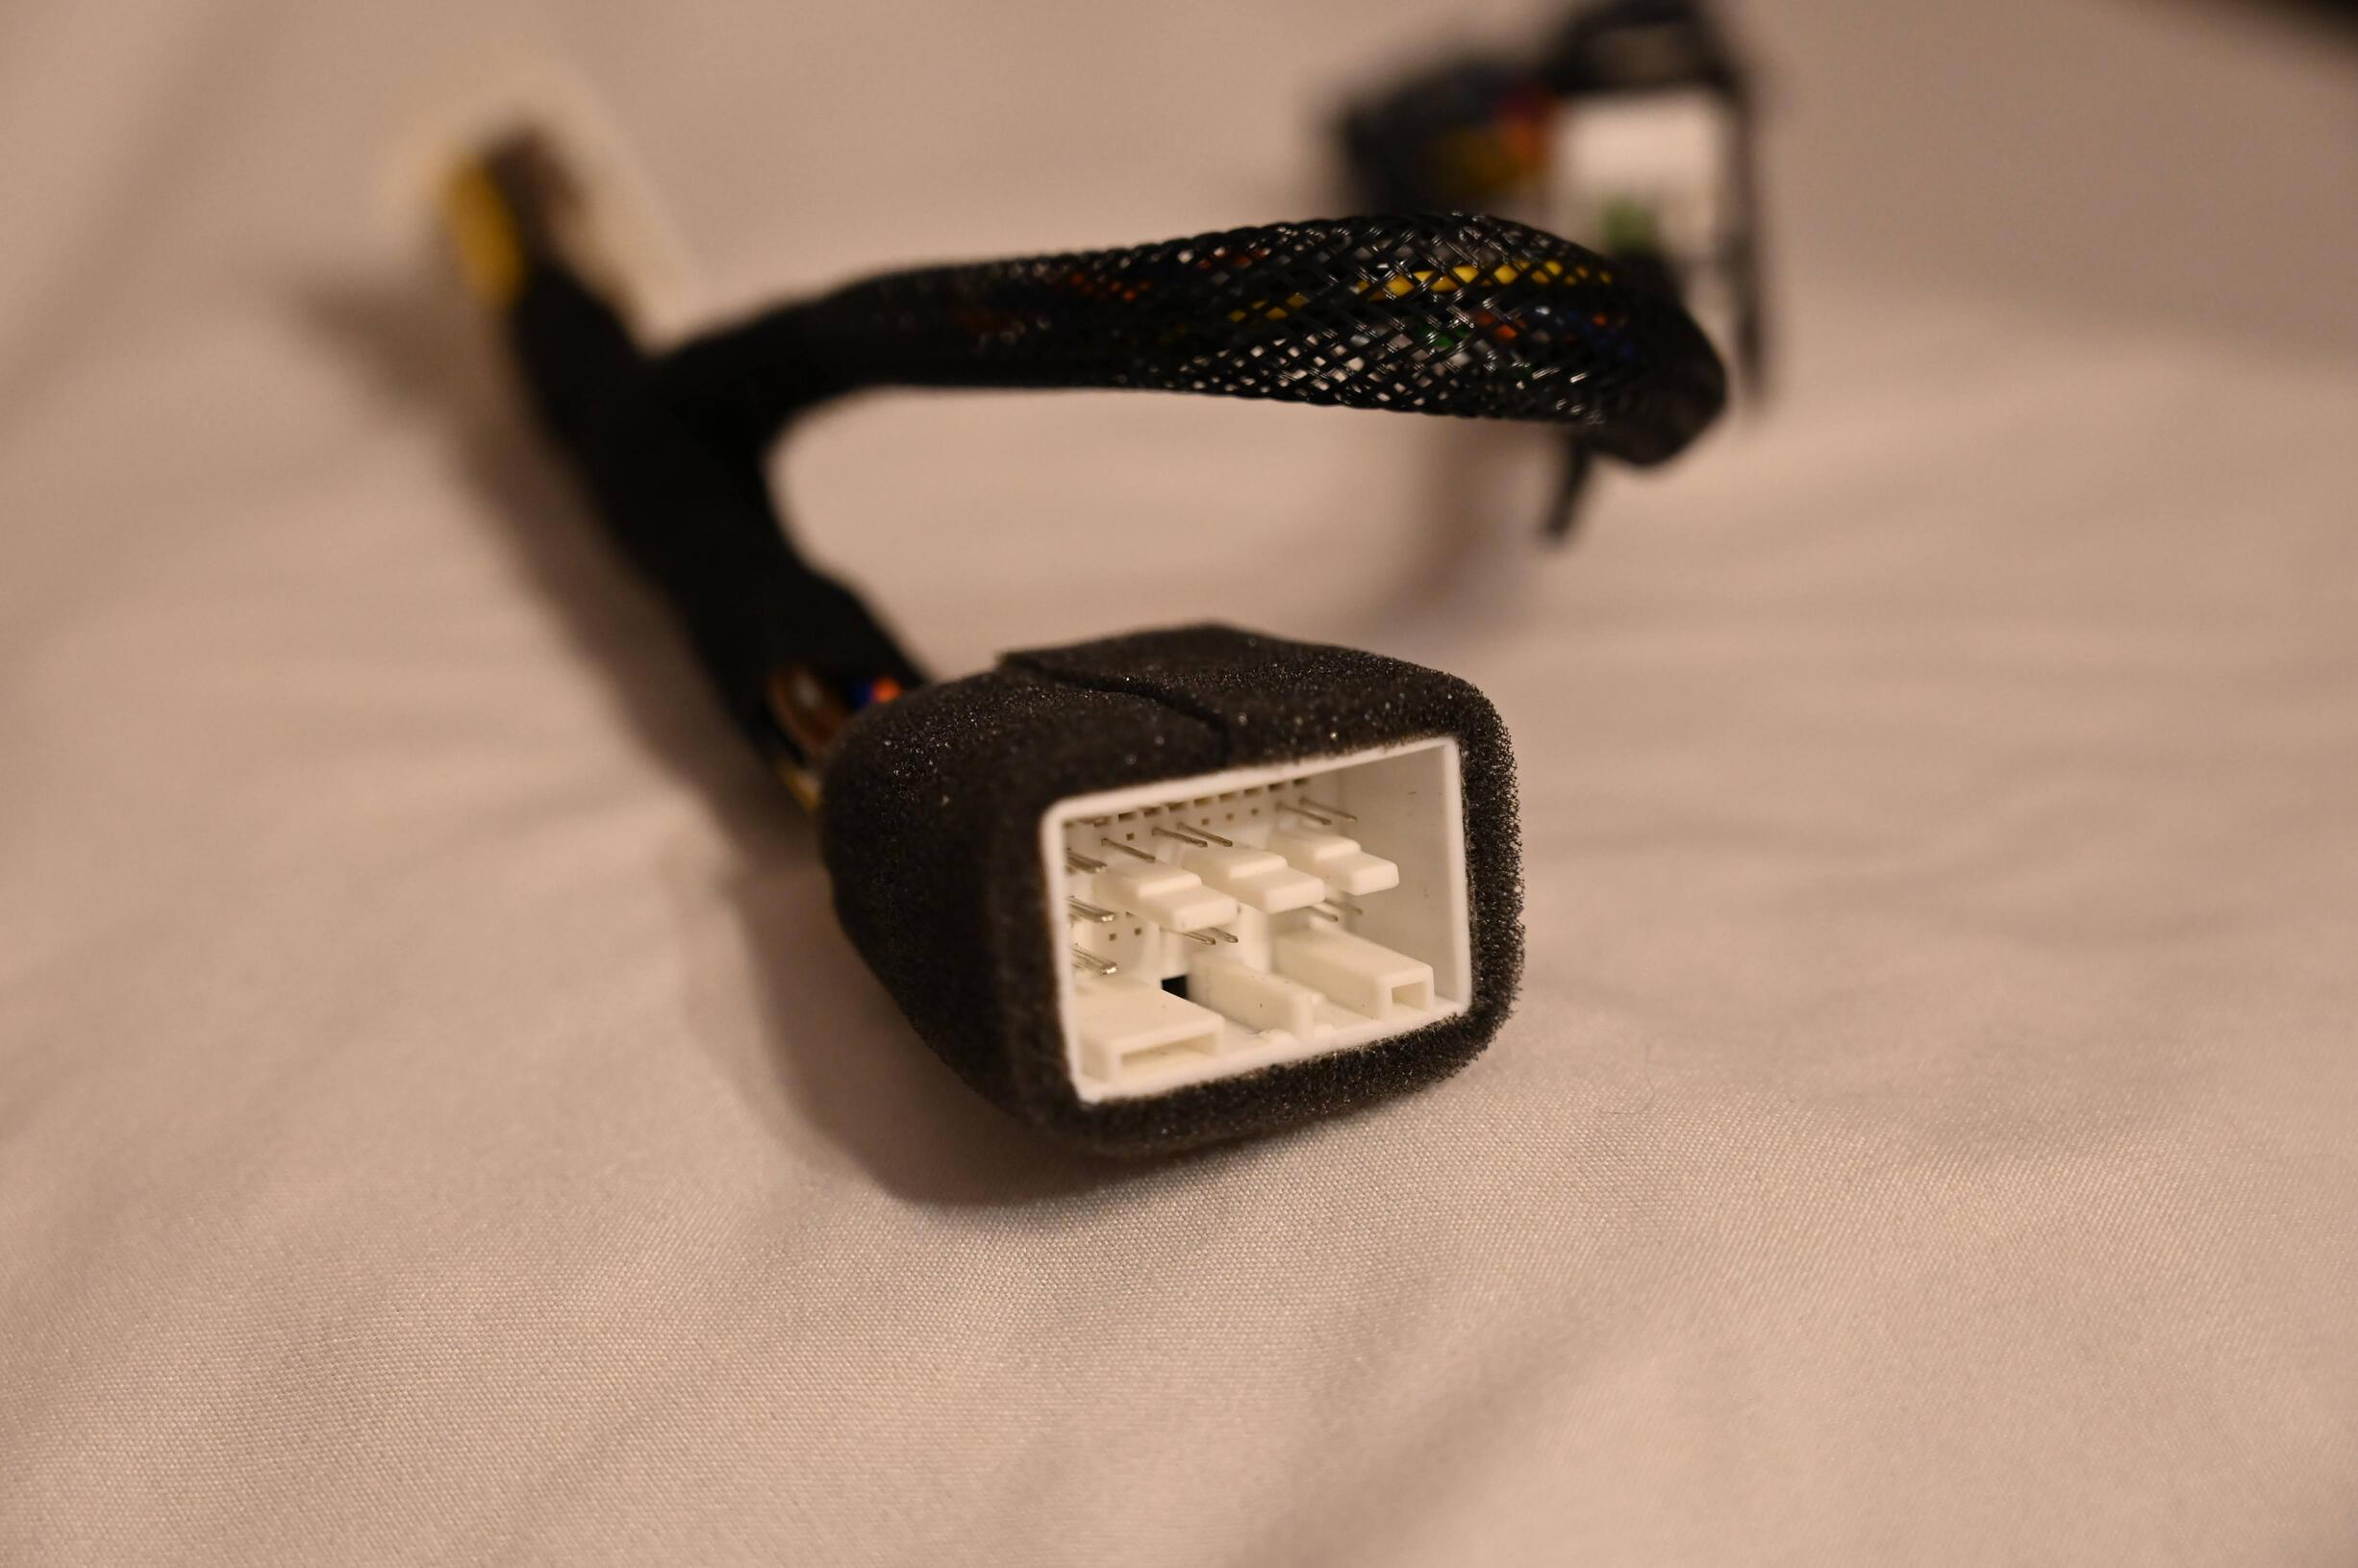
\includegraphics[height=1.5in,angle=0]{../Ioniq5/photos/male_harness_end.jpg} }  \\
  \subfloat[]{\label{subfig:harness:headunit_oe_connectors}
  \includegraphics[height=1.5in,angle=0]{photos/HU_dangling_clip_detached.jpg} } 
  \subfloat[]{\label{subfig:harness:harness_male_in}
  \includegraphics[height=1.5in,angle=0]{photos/harness_installing_3.jpg} } 
  \subfloat[]{\label{subfig:harness:harness_in}
  \includegraphics[height=1.5in,angle=0]{photos/HU_dangling_clip_detached_2.jpg} }  
   \caption{(a) Photo étiquetée montrant le connecteur de faisceau femelle. (b) Connecteur de faisceau mâle. (c) Unité principale avec les connecteurs d'origine branchés. (d) Connecteur femelle (gris) retiré de l'unité principale. (e) Harnais installé dans l'unité principale. \label{fig:harness}}
\end{figure}
\section{Étape 4 : Montage OBD} \label{sect:3}
Dans cette étape, nous montons solidement l’extrémité OBD du faisceau et branchons le WiCAN. 

Instructions étape par étape :
\begin{enumerate}
  \item Filetage de l'extrémité OBD sur le support de montage de l'unité principale (Figure \ref{subfig:obd:thread_obd})
  \item Remontez l’unité principale. (Chiffre \ref{subfig:trim:HU_screws})
  \item Branchez la prise OBD femelle dans le support fourni, si ce n'est déjà fait.
  \item Utilisez du ruban adhésif double face pour monter le support sur une surface plane
  \item Utilisez des attaches zippées pour attacher le faisceau à d'autres fils et points de montage 
  \item Tout en tenant le support, branchez le WiCAN (Figure \ref{subfig:obd:wican})
\end{enumerate}

\begin{figure}[h]
  \subfloat[]{\label{subfig:obd:thread_obd}
  \includegraphics[height=1.5in,angle=0]{photos/harness_installed_HU_detached.jpg} }  
  \subfloat[]{\label{subfig:obd:installed}
  \includegraphics[height=1.5in,angle=0]{photos/harness_installed_1.jpg} } 
  \subfloat[]{\label{subfig:obd:wican}
  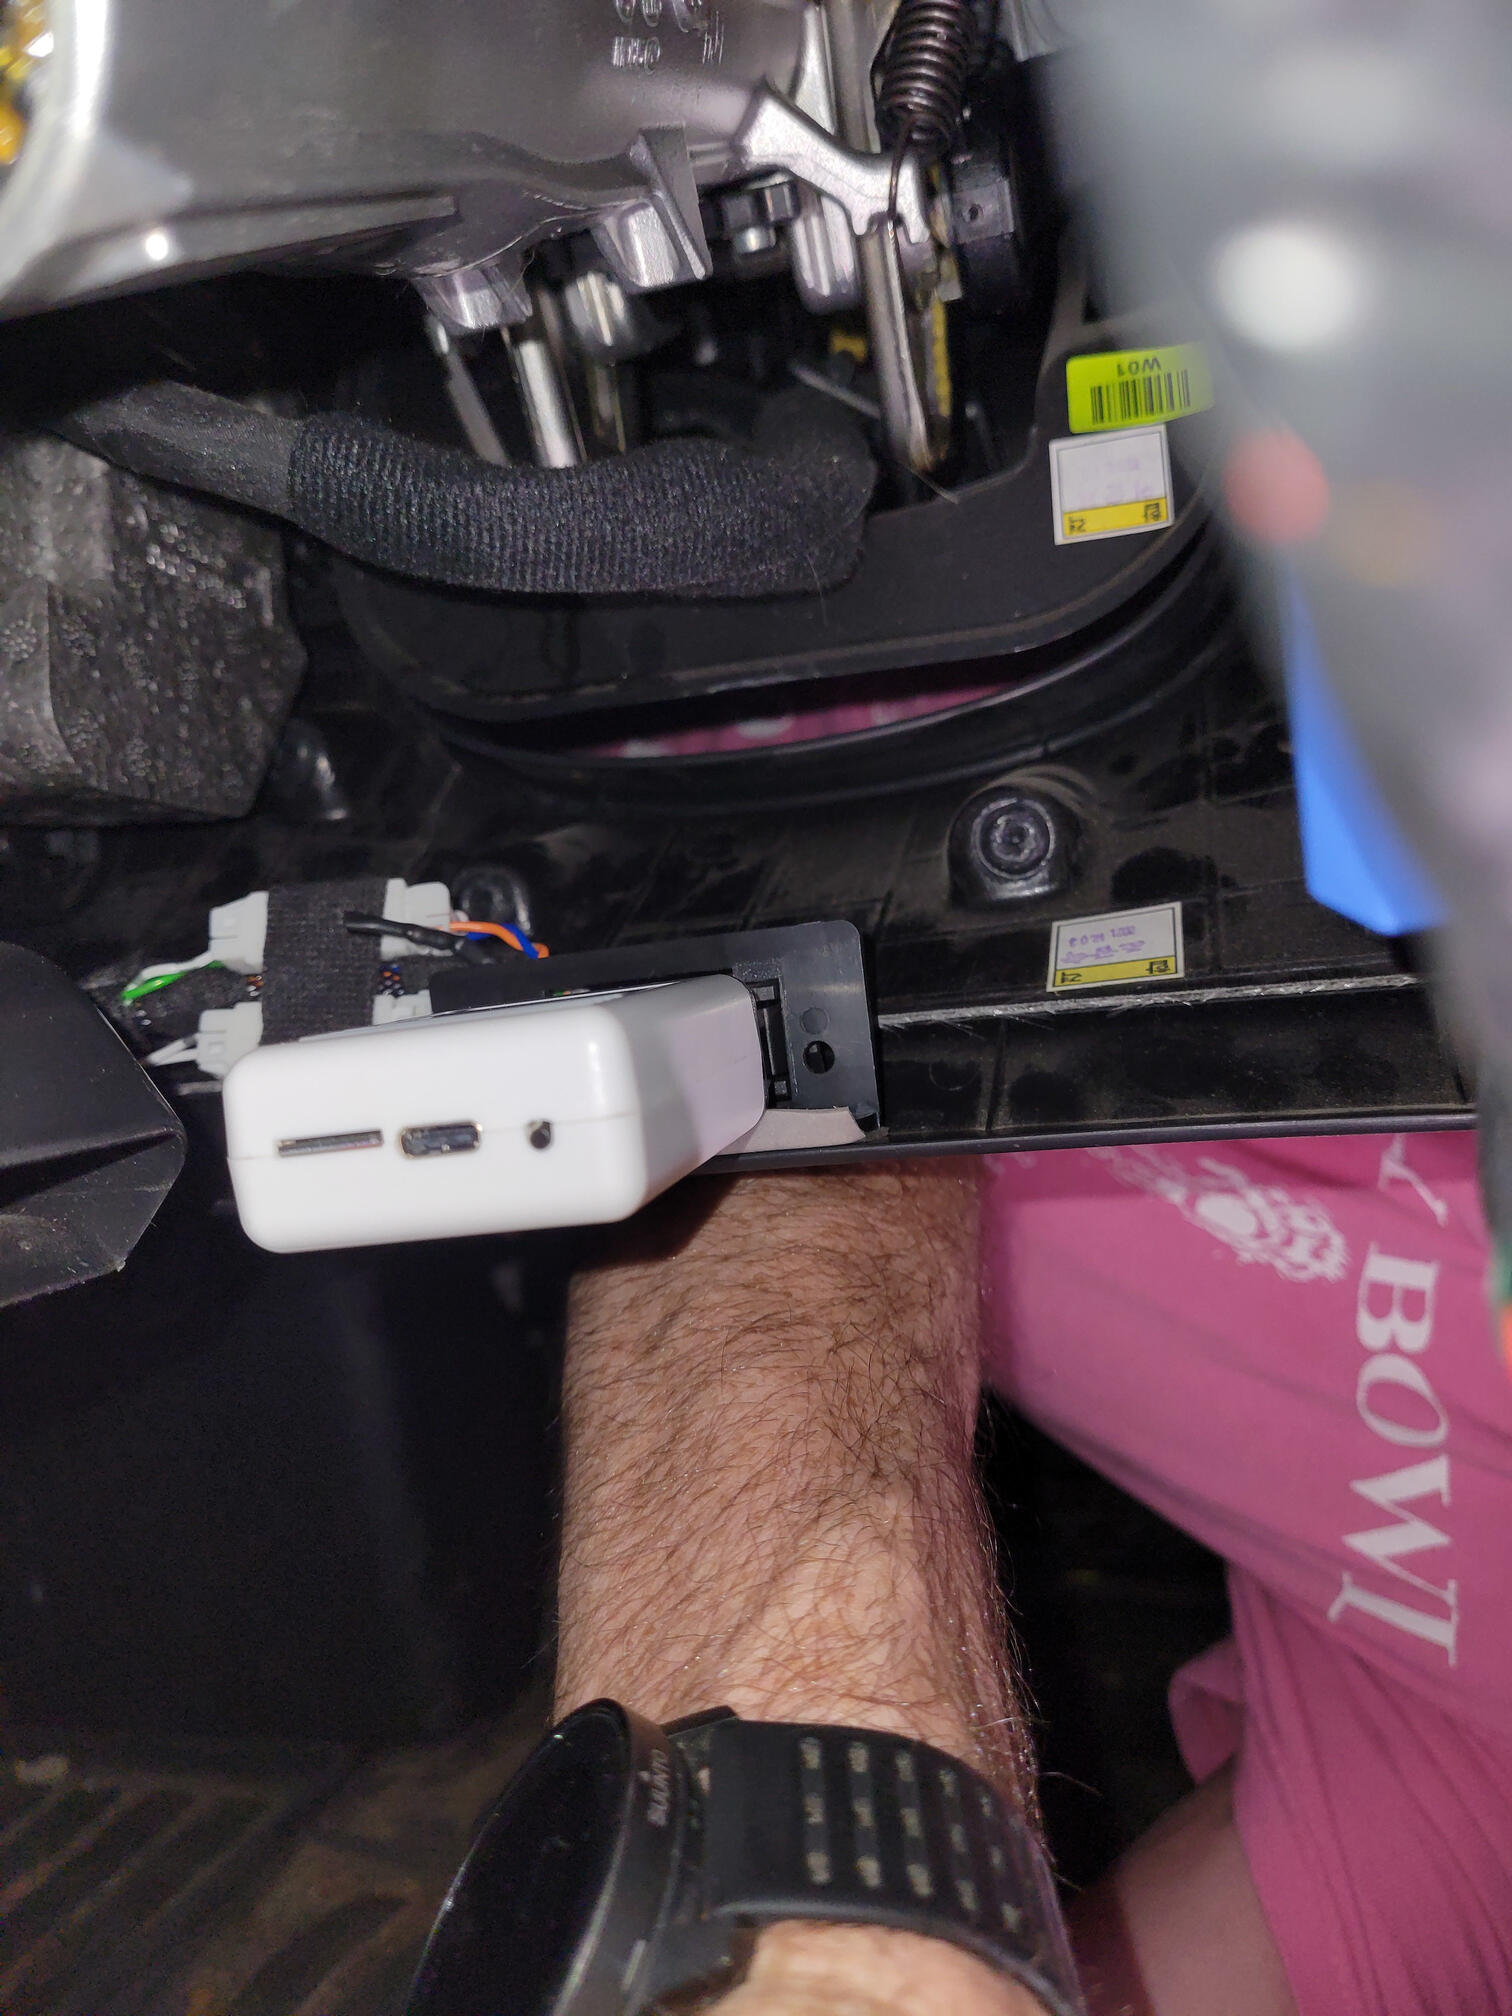
\includegraphics[height=1.5in,angle=0]{../Ioniq5/photos/wican_inserted.jpg} } 
   \caption{(a) Support de montage de l'unité principale fileté OBD. (b) Harnais attaché au fil existant. (c) WiCAN inséré dans l'OBD. \label{fig:obd}}
\end{figure}

\section{Étape 5 : Nettoyer} \label{sect:4}
Inversez les étapes de retrait des garnitures. Assurez-vous que les clips de garniture sont alignés, puis remettez fermement les panneaux de garniture en place. Rebranchez la borne négative de la batterie 12 V. Le WiCAN devrait immédiatement afficher une lumière bleue. Changez votre mot de passe WiCAN : \href{https://meatpihq.github.io/wican-fw/config/wifi}{https://meatpihq.github.io/wican-fw/config/wifi}. Vous pouvez connecter votre WiCAN directement en trouvant un réseau WiFi nommé 'WiCAN\_xxxxxxx' et je vais à \href{http://192.168.80.1/}{http://192.168.80.1/} dans votre navigateur.
% \appendix 
\end{document}